% !TEX encoding = UTF-8 Unicode
%%%%%%%%%%%%%%%%%%%%%%%%%%%%%%%%%%%%%%%%%
% Journal Article
% LaTeX Template
% Version 1.4 (15/5/16)
%
% This template has been downloaded from:
% http://www.LaTeXTemplates.com
%
% Original author:
% Frits Wenneker (http://www.howtotex.com) with extensive modifications by
% Vel (vel@LaTeXTemplates.com)
%
% License:
% CC BY-NC-SA 3.0 (http://creativecommons.org/licenses/by-nc-sa/3.0/)
%
%%%%%%%%%%%%%%%%%%%%%%%%%%%%%%%%%%%%%%%%%

%----------------------------------------------------------------------------------------
%	PACKAGES AND OTHER DOCUMENT CONFIGURATIONS
%----------------------------------------------------------------------------------------
\documentclass[oneside, 11 pt]{article}
\usepackage[utf8]{inputenc}
\usepackage[T1]{fontenc}
\usepackage{textcomp}
\usepackage[portuguese]{babel}
\usepackage{blindtext} % Package to generate dummy text throughout this template 
\usepackage{comment}
\usepackage{listings}
\usepackage{xcolor}
\usepackage{hyperref} % For hyperlinks in the PDF

\usepackage{inconsolata}
\lstset{
	language=bash, %% Troque para PHP, C, Java, etc... bash é o padrão
	basicstyle=\ttfamily\small,
	numberstyle=\footnotesize,
	backgroundcolor=\color{gray!10},
	frame=single,
	tabsize=2,
	rulecolor=\color{black!30},
	escapeinside={\%*}{*)},
	breaklines=true,
	breakatwhitespace=true,
	framextopmargin=2pt,
	framexbottommargin=2pt,
	inputencoding=utf8,
	extendedchars=true,
	literate={á}{{\'a}}1 {ã}{{\~a}}1 {é}{{\'e}}1 {í}{{\'i}}1,
}
\usepackage[hmarginratio=1:1,top=32mm,columnsep=20pt]{geometry} % Document margins
\usepackage[hang, small,labelfont=bf,up,textfont=it,up]{caption} % Custom captions under/above floats in tables or figures
\usepackage{booktabs} % Horizontal rules in tables

\usepackage{lettrine} % The lettrine is the first enlarged letter at the beginning of the text

\usepackage{enumitem} % Customized lists
\setlist[itemize]{noitemsep} % Make itemize lists more compact

\usepackage{titlesec} % Allows customization of titles
%\renewcommand\thesection{\Roman{section}} % Roman numerals for the sections
%\renewcommand\thesubsection{\roman{subsection}} % roman numerals for subsections
\titleformat{\section}[block]{\large\scshape\centering}{\thesection.}{1em}{} % Change the look of the section titles
\titleformat{\subsection}[block]{\large}{\thesubsection.}{1em}{} % Change the look of the section titles

\usepackage{fancyhdr} % Headers and footers
\pagestyle{fancy} % All pages have headers and footers
\fancyhead{} % Blank out the default header
\fancyhead[C]{Terceiro Exercício prático de Bash} % Custom header text

\usepackage{titling} % Customizing the title section

\usepackage{graphicx}
\usepackage{float}
\renewcommand{\arraystretch}{1.5}
\usepackage{multirow}
\setlength{\parindent}{18pt}
\setcounter{secnumdepth}{0}

\usepackage{xcolor}
\hypersetup{
	colorlinks,
	linkcolor={red!60!black},
	citecolor={blue!50!black},
	urlcolor={blue!80!black}
}
%----------------------------------------------------------------------------------------
%	TITLE SECTION
%----------------------------------------------------------------------------------------

\setlength{\droptitle}{-4\baselineskip} % Move the title up

\pretitle{\begin{center}\Huge\bfseries} % Article title formatting
	\posttitle{\end{center}} % Article title closing formatting
\title{Terceiro Exercício prático de Bash} % Article title
\author{%
	\textsc{Guilherme Bittencourt Bueno da Silva} \\[1ex] % Your name
	\normalsize Universidade Federal do Paraná \\ % Your institution
	\normalsize {gbbs14@inf.ufpr.br} % Your email address
	%\and % Uncomment if 2 authors are required, duplicate these 4 lines if more
	%\textsc{Jane Smith}\thanks{Corresponding author} \\[1ex] % Second author's name
	%\normalsize University of Utah \\ % Second author's institution
	%\normalsize \href{mailto:jane@smith.com}{jane@smith.com} % Second author's email address
}
\date{\today} % Leave empty to omit a date
\renewcommand{\maketitlehookd}{%
	
	%\begin{abstract}
	%\noindent \blindtext % Dummy abstract text - replace \blindtext with your abstract text
	%\end{abstract}
}

%----------------------------------------------------------------------------------------

\begin{document}
	
	% Print the title
	\maketitle
	
	%----------------------------------------------------------------------------------------
	%	ARTICLE CONTENTS
	%----------------------------------------------------------------------------------------
	\section{Resumo}
	O exercício a seguir propõe ao leitor encontrar uma solução rápida para analiser o log de um firewall, enviando e-mail caso alguma filtragem tenha muitas ocorrências e redirecionando a solução para um arquivo com nome relativo à data e versão da análise. A solução inclui a pesquisa por ferramentas que possam ser de auxílio na solução como o awk, grep entre outros.
	
	\section{Introdução}
	logs são uma fonte bem comum de dado para scripts, contendo texto em ASCII e um separador único para colunas. Logs são gerados automaticamente por algum sistema, com alguma periodicidade, portanto é comum identificar a saída de um script, que executa sobre um log, com um timestamp no nome.  O exercício a seguir exige uma contagem rápida passando por todas as linhas de um log. A solução apresentada nesse material utiliza o awk para realizar a operação principal, devido ao seu fluxo linha por linha.
	
	\section{Exercício}
	Cada linha do log pode ter uma quantidade diferente de colunas, separadas por espaço. Os tipos de filtragem sempre se encontram na 6ª coluna. As linhas não estão ordenadas por tipo de bloqueio.
	
	\begin{figure}[h]
		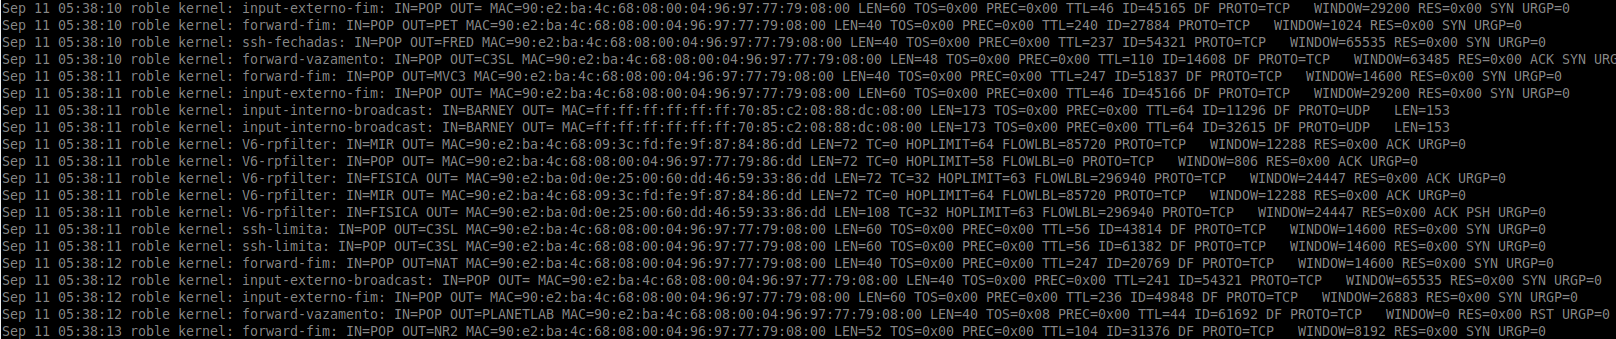
\includegraphics[width=\linewidth]{loglines.png}
		\caption{Exemplo de linhas do log}
		\label{fig:loglines}
	\end{figure}

	\pagebreak
	
	Todos os tipos de filtragem existentes se encontram em um arquivo "tipos-bloqueios", no formato:
	
	\begin{lstlisting}
	...
	V6-windows
	bios_debian
	bogon
	dns
	forward-fim
	forward-syn-piratas
	forward-vazamento
	input-externo-broadcast
	input-externo-fim
	...
	\end{lstlisting}
	
	O exercício consiste em fazer um script que retorne uma lista de tipos de bloqueios e suas ocorrências a partir de um log no formato descrito acima. A saída deve ser redirecionada para um arquivo contendo a data atual no nome. O script deve receber um parâmetro de versão. Versão V6, deve considerar todos os tipos de bloqueio que começam com "V6", versão "V4", deve considerar todos os tipos de bloqueios que \textbf{não} começam com "V6". Caso não receba nenhum argumento, todos os tipos de bloqueios devem ser considerados. O parâmetro de versão também deve ser identificado no nome do arquivo gerado. Os bloqueios sem nenhuma ocorrências devem aparecer no resultado. Caso um ou mais tipos de bloqueio tenham mais de 20000 ocorrências, o script deve enviar um e-mail com esses tipos de bloqueios e a quantidade de ocorrências de cada um deles.
	
	\pagebreak
	
	\section{Solução}
	
	\begin{lstlisting}
	1 #!/bin/bash
	2 
	3 # "Versão" sem o "-"
	4 ver=${1:1:2};
	5 # Organiza logs criados pela data e versão
	6 logn="log-$(date | awk -F " " '{print $3 $2 $6}')$ver";
	7 if [ -f $logn ]; then
	8     rm $logn;
	9     touch "$logn";
	10 fi
	11 
	12 if [ "$1" == "-V6" ]; then
	13     bloqTypes=$(grep "V6" tipos-bloqueios | tr "\n" " ");
	14 elif [ "$1" = "-V4" ]; then
	15     bloqTypes=$(grep "V6" -v tipos-bloqueios | tr "\n" " ");
	16 else
	17     bloqTypes=$(cat tipos-bloqueios | tr "\n" " ");
	18 fi
	19 
	20 mail=$(awk -v types="$bloqTypes" -v logn="$logn" '
	21 {countTypes[substr($6, 1, length($6)-1)] += 1}
	22 END {
	23     split(types, tps, " ");
	24     count = 1;
	25     for (tp in tps)
	26     {
	27         print tps[tp],":",(tps[tp] in countTypes) ? countTypes[tps[tp]] : 0 >> logn;
	28         if (countTypes[tps[tp]] > 20000)
	29         {
	30             print tps[tp], countTypes[tps[tp]];
	31         }
	32     }
	33 }
	34 ' log-firewall);
	35 
	36 echo "$mail" | mail -s "firewall warning $logn" gbbs14@inf.ufpr.br;
	\end{lstlisting}
	
	As linhas 3-10 servem para criar o log com o nome no formato: log-[data][versão]. Na linha 4, a variável \texttt{\textbf{\textit{ver}}} recebe o conteúdo dos índices 1 a 2 do primeiro parâmetro \texttt{\textbf{\textit{\$1}}}. Ou seja, removendo o índice 0, que contém o "-", restando apenas V6 ou V4. A data é obtida pelo comando "date", utilizando o awk para selecionar os campos necessários. Caso já exista um log com o nome gerado no diretório atual, ele é apagado, pois o resultado é inserido nesse arquivo linha por linha, com ">>", sem sobrescrever o conteúdo anterior.
	
	Nas linhas 12 a 18, os tipos de bloqueio são passados para a variável \texttt{\textbf{\textit{fileItemString}}} de acordo com a versão selecionada. A troca de \textbackslash n por espaços é necessária para que a cada elemento do array \texttt{\textbf{\textit{fileItemString}}} receba uma linha do resultado do grep.
	
	Na linha 20, o awk é invocado, com seu resultado sendo redirecionado à variável mail. Isso porque, dentro do awk, o real resultado será redirecionado ao arquivo criado no início do script, sendo assim, ainda é possível aproveitar o retorno do awk para retornar o conteúdo do email a ser enviado. São delclaradas 2 variáveis para o awk, contando os tipos a serem contados e nome do arquivo que deve receber o resultado.
	
	O fluxo principal do awk está na linha 21. Para cada linha, o array associativo \texttt{\textbf{\textit{countTypes}}}, é incrementado em cada índice. O índice é a substring da sexta coluna, removendo o último caractere, que em todos os casos é um ":". Note que não é necessário inicializar cada valor, dessa forma, ao final do arquivo, o array \texttt{\textbf{\textit{counTypes}}} contém todos os tipos de bloqueio como índice (incluíndo os tipos de bloqueio que não devem ser impressos no resultado, se houver), associados à quantidade de ocorrências de cada um deles.
	
	Ao final da execução principal do arquivo, no awk, nas linhas 22 a 33, para cada tipo de bloqueio (entre os bloqueios necessários para a versão escolhida), são impressos o índice associativo (tipo de bloqueio) da variável \texttt{\textbf{\textit{countTypes}}} e seu valor associado (quantidade de ocorrências) e se houverem mais de 20000 ocorrências desse tipo de bloqueio, esses valores são impressos ao retorno do awk (que no caso, é a variável mail).
	
	Na linha 36, um echo da variável \texttt{\textbf{\textit{\$mail}}} é usado como conteúdo do email, redirecionado ao comando mail. O campo assunto contém o nome do arquivo de retorno, que possui a data e versão da execução do script.
	
	\begin{figure}[h]
		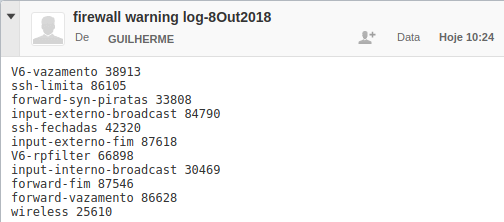
\includegraphics[width=\linewidth]{mail.png}
		\caption{Exemplo de Email enviado}
		\label{fig:mail}
	\end{figure}
	
	\section{Conclusão}
	Para otimizar o desempenho, o script conta todos os tipos de bloqueio, independente de quais tipos de bloqueios serão impressos no resultado, assim, evitando branches no loop principal, que é na linha 21, onde o awk percorre cada linha do arquivo.
	

%----------------------------------------------------------------------------------------
%   REFERENCE LIST
%----------------------------------------------------------------------------------------
\end{document}